%Exp 1-8
\chapter{Centripetal Force and Angular Momentum Conservation}
\label{chap:centripetal}
\section{Introduction}
In this experiment, we study the same concepts of rotational motion covered in experiment 1-6. Specifically, we study conservation of {\it{angular}} momentum and the rotational equivalent of Newton's second law as it pertains to centripetal acceleration. The purpose of this experiment is two-fold: to examine centripetal force by studying the effects of varying the mass of the object, the radius of the circle, and the centripetal force on an object rotating in a circular path; and to examine angular momentum conservation by observing the effect of changing the rotational inertia of the system without exerting torque on the system.

\section{Theory}
\subsection{Centripetal Force}
When an object of mass $M$ is rotated in a horizontal circle of radius $r$ (so that gravitational energy remains constant throughout the motion), the centripetal force on the mass is given by:

\begin{equation}
\vec F = - \frac{M v^{2}}{r} \vec {\hat r} =- M \vec r \omega ^2
\end{equation}

\noindent where $\vec v$ and $\vec \omega$ are the the tangential and angular velocities, respectively ($|v| = r |\omega|$).

\subsection{Angular Momentum Conservation}
\noindent{ If you recall from linear Newtonian motion, when no external forces act on a system, the total linear momentum of the system is constant. A similar statement can be said for {\it{rotational}} motion. When no external {\it{torques}} act on a system, the total {\it{angular}} momentum is constant. During the angular momentum portion of the experiment a ring will be dropped onto a rotating disk, thereby changing the system's rotational inertia. Since there is no net torque on the system, there is no change in angular momentum. Angular momentum is conserved}

\begin{equation}
\vec L = I_{i} \vec \omega _{i} = I_{f} \vec \omega _{f}
\end{equation}

\noindent{where $I_{i}$ is the initial rotational inertia and $\omega _{i}$ is the initial angular speed, while $I_{f}$ is the final rotational inertia and $\omega _{f}$ is the final angular speed. The initial rotational inertia is that of a disk, whereas the final rotational inertia is that of a disk {\it{and}} a ring.}

\begin{equation}
I_{i} = \frac{1}{2}M_{1}R^{2}
\end{equation}

\noindent{where $M_{1}$ is the mass of the disk and $R$ is its radius.  The final rotational inertia $I_{f}$ is the combination of a disk and a ring}

\begin{equation}
I_{f} = \frac{1}{2}M_{1}R^{2} + \frac{1}{2}M_{2}(r_{1}^{2} + r_{2}^{2})
\end{equation}

\noindent{where $M_{2}$ is the mass of the ring and $r_{1}$ and $r_{2}$ are the inner and outer radii of the ring, respectively.}\myskip


\section{Procedure}
\begin{figure}[!h]
	\begin{center}
	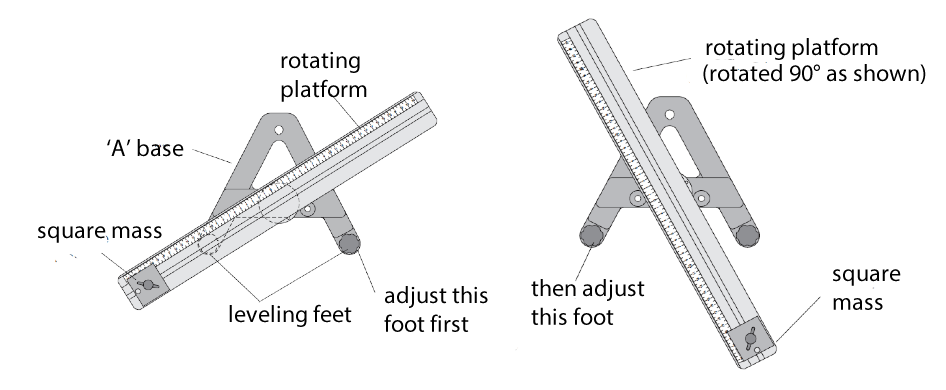
\includegraphics[width=0.8\textwidth]{./Exp1-8/pic/appbalance2.png}
	\end{center}
\caption{Diagram explaining the procedure for leveling the rotating apparatus.}
\label{fig:levelapp1}
\end{figure}
\begin{figure}[h]
	\begin{center}
	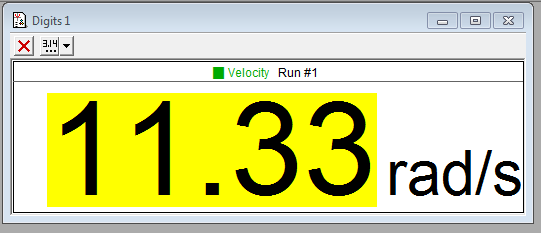
\includegraphics[width=0.5\textwidth]{./Exp1-8/pic/screenshot1.png}
	\end{center}
\caption{The digit display of instantaneous angular frequency in DataStudios.}
\label{fig:screen1}
\end{figure}
\subsection{Level the apparatus.}
The accuracy of this experiment requires the apparatus to be extremely level. To level the base, perform the following steps:

\begin{enumerate}
	\item Set up the apparatus with the mass hanging from the sidepost, the clamp-on pulley attached to the end near the side post, and the spring at the center post (but no mass hanging on the pulley), level the apparatus as was done in the previous Rotational Inertia Experiment:
	\item Rotate the track until the clamp-on pulley end of the track  is above the left foot of the ``A'' base. See the left side of Figure \ref{fig:levelapp1} (where the ``square mass" in this case is the  clamp-on pulley end).
	\item Adjust the leveling screw on the side opposite the pulley until the end of the track with the clamp-on pulley  is aligned over the leveling screw on the other leg of the base. See the left side of Figure \ref{fig:levelapp1}.
	\item Rotate the track 90 degrees so it is parallel to the right side of the ``A" and adjust the opposite leveling screw until the track is stable in the parallel position. See the right side of Figure \ref{fig:levelapp1}.
	\item The track should now be level and it should remain at rest regardless of its orientation.
\end{enumerate}

\subsection{Centripetal Force}
\subsubsection{Vary Radius (constant force and mass)}
\label{varyr}
\noindent The centripetal force and the mass of the hanging object will be held constant for this part of the experiment. The purpose of steps 1-9 are to calibrate the system to a constant, measurable centripetal force . Steps 10-23 are measuring the relation between the radius of the side post and the angular velocity of the side post using the centripetal force set by steps 1-9.

\begin{enumerate}
	\item Weigh the mass hanging from the side post and record its mass $M$ in Table \ref{resultstable}.
	\item Reattach the hanging mass and connect the string from this mass to the spring hanging from the center post through the center pulley. The string must pass under the pulley on the center post. See Figure \ref{fig:apparatus}.
	\item Move the center post so that it is at the center of the track (0 cm). This can be done by loosening the knob, moving the post and retightening.
	\item Attach a string to the hanging object and hang a known mass over the clamp-on pulley. Record this mass $m$ in Table \ref{resultstable}. This establishes the constant centripetal force.
	\item Adjust the position of the side post to be approximately three-quarters of the way between the center post and the clamp-on pulley by pressing down on the side post to assure that it is vertical, then tightening the thumb screw on the side post to secure its position.
	\item The distance between the center post and the side post (measured using the scale on the track) determines the initial radius $r$. Record this radius $r$ in the first row of Table \ref{datatable}.
	\item The object on the side post must hang vertically. Adjust the spring bracket vertically, by loosening the knob at the top of the center post and moving it up or down to vary the stretching of the spring, until the string from which the object hangs on the side post is aligned with the vertical line on the side post. If this is infeasible with the current setup, either lengthen or shorten the string as necessary or reposition the sidepost.
	\item Align the ring indicator bracket on the center post so that it is centered on the orange indicator on the spring.
	\item Remove the mass that is hanging from the clamp-on pulley.
	\item Start the ``Centripetal Force" DataStudio program.
	\item Rotate the apparatus gently by hand (attempting not to jostle the mass hanging from the side post), increasing the rotation speed until the orange indicator on the spring is again centered with the ring indicator bracket on the center post. This indicates that the centripetal force acting on the mass hanging from the side post is now equivalent to the force that was previously imparted by the mass hanging from the clamp-on pulley.
	\item Record this angular speed (when the orange indicator is centered in the ring indicator) from the software (see Figure \ref{fig:screen1}).
	\item Record the angular speed and the radius of the side post in the first row of Table \ref{datatable}.
	\item Move the side post to a new radius and repeat steps 1-13. Do this for a total of five radii.
	\item Calculate the inverse of the square of the angular velocity $1/\omega^2$ for each trial and record these values in Table \ref{datatable}.
	\item The weight of the mass hanging from the clamp-on pulley is equal to the centripetal force applied by the spring. Calculate this force by multiplying the mass hung from the clamp-on pulley by $g = 9.81$ m/s$^{2}$ and record this force $mg$ in Table \ref{resultstable}.
	\item In Excel, plot the radius $r$ on the vertical axis versus the inverse square of the angular velocity $1/\omega^2$ on the horizontal axis for all five data points. This should give a straight line since:
	\begin{equation}
		r = \frac{|F|}{M}\frac{1}{\omega^2}
	\label{eq:rvsomegasq}
	\end{equation}
	\item Include error bars on both axes of your plot. Error in radius $r$ can be found from the precision of the ruler. Error in $\omega^2$ can be found by propagating uncertainty in $\omega$. Uncertainty in $\omega$ can be found from the precision of the DataStudios program.
	\item Determine the best-fit line through the data points using Excel and record the slope of the line (which equals $F/M$).
	\item Calculate the uncertainty in your measured slope using the LINEST function. Record the slope with error in Table \ref{resultstable}
	\item Calculate the centripetal force $F$ with error from the slope using Equation \ref{eq:rvsomegasq}
 and record the result in Table \ref{resultstable}.
	\item Calculate a percent difference between the centripetal force determined from $mg$ and from the slope $F$.  Record this percent difference in Table \ref{resultstable}.
	\item Is the force found from the slope within uncertainty of the force determined by the mass hanging from the clamp-on pulley when the system was not in rotation?
	\item Discuss the main sources of error in this experiment.
\end{enumerate}

\begin{figure}[h]
	\begin{center}
	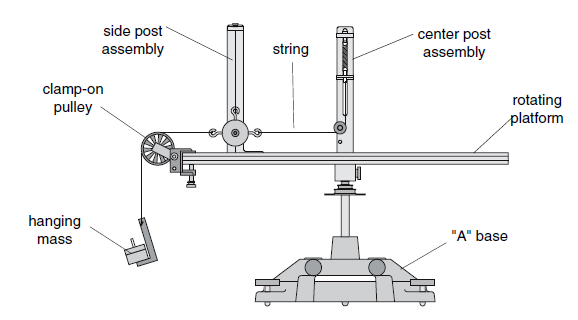
\includegraphics[width=0.7\textwidth]{./Exp1-8/pic/apparatus.png}
	\end{center}
	\caption{The centripetal force apparatus}
	\label{fig:apparatus}
\end{figure}

\newcolumntype{C}[1]{>{\centering\let\newline\\\arraybackslash\hspace{0pt}}m{#1}}



\subsection{Conservation of Angular Momentum}
\label{diskinert}
\begin{enumerate}
	\item Remove the track used in the previous experiment and position the rotational disk directly on the center shaft as shown in Figure \ref{fig:rotinert}.  The side of the disk that has the indentation for the ring should be up.
	\item Spin the disk with your hand.
	\item Start recording data using the "Centripetal Force" DataStudio program.  After approximately 25 data points have been taken, carefully drop the mass ring onto the spinning disk so that it rests on the indentation. Stop recording data a few seconds after the mass ring is dropped on the disk.
	\item Use the velocity graph to determine the angular speed right before the collision ($\omega _{i}$) and right after the collision ($\omega _{f}$).
	\item Repeat for 3 trials and enter data into Table \ref{eightab}.
	\item Calculate the initial and final moments of inertia $I$, using the appropriate expressions for $I$ for the disk and the ring. You may need to measure their masses and radii. Include error in calculated moments of inertia $I$ by propagating uncertainty in measured radius $r$.
	\item Calculate initial and final angular momenta $L$, by multiplying moments of inertia $I$ by the relevant initial and final angular velocities. Include error in angular momentum $L$ by propagating uncertainties in moment of inertia $I$. Enter these values with error into Table \ref{eightab}.
	\item Calculate the ratio of the initial angular momentum to the final angular momentum ($R = |L_i| /|L_f|$) for all three trials. Calculate the uncertainty in $R$ by propagating uncertainties in angular momentum.
	\item Is angular momentum conserved within error? What value of $R$ should we get if angular momentum is conserved?
	\item Why might angular momentum not be conserved (think about the assumption of angular momentum conservation)?
	\item  What are the main sources of error? Which source of error do you think dominates in this experiment?
\end{enumerate}

\begin{figure}[h]
	\begin{center}
		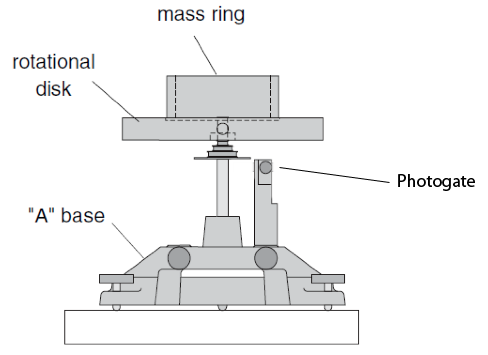
\includegraphics[width=0.6\linewidth]{./Exp1-8/pic/othersetup.png}
	\end{center}
	\caption{The conservation of angular momentum setup mentioned in Section \ref{diskinert}}
	\label{fig:rotinert}
\end{figure}

\begin{table}[h]
\begin{center}
\begin{tabular}{| C{4.5 cm} | C{4.5 cm} | C{4.5 cm} |}
\hline
	$r$ (cm) & $\omega$ (rad/s) & $\frac{1}{\omega ^{2}}$ (s$^{2}$/rad$^{2}$)\\
	\hline
	& & \\
	\hline
	& & \\
	\hline
	& & \\
	\hline
	& & \\
	\hline
	& & \\
	\hline
\end{tabular}
\end{center}
\caption{Angular velocities $\omega$ for various radii $r$.}
\label{datatable}
\end{table}
\begin{table}[!h]
\begin{center}
\begin{tabular}{| C{9 cm} | C{5 cm} |}
	\hline
	{\bf{Mass hanging from side post $= M$}} & \\
	\hline
	{\bf{Mass hanging from clamp-on pulley $= m$}} & \\
 	\hline
	{\bf{Centripetal force $ = mg$}} & \\
	\hline
	{\bf{Slope from graph $= F/M$}} & \\
	\hline
	{\bf{Centripetal force from slope $= F$}} & \\
	\hline
	 {\bf{Percent difference between $mg$ and $F$}} & \\
	\hline
\end{tabular}
\end{center}
\caption{Results for Section \ref{varyr}.}
\label{resultstable}
\end{table}
\begin{table}[!h]
\centering
\begin{tabular}{| C{2.5cm} | C{2.5 cm} | C{2.5 cm} | C{2.5 cm} | C{2.5 cm} |}
\hline
$\omega _{i}$ (rad/s) & $\omega _{f}$ (rad/s) & $L_{i}$ (kg.m$^{2}$/s) & $L_{f}$ (kg.m$^{2}$/s)  & $R$\\ \hline
& & & & \\ \hline
& & &  & \\ \hline
& & & & \\ \hline
\end{tabular}\\
\caption{Angular velocities and angular momenta before and after collision.}
\label{eightab}
\end{table}
